\begin{figure}[h]
  \vspace{4mm}
  \centering
\usetikzlibrary{matrix, positioning,backgrounds,arrows.meta, arrows, decorations.markings}
\tikzstyle{vecArrow}[black] = [thick, #1, decoration={markings,mark=at position
    1 with {\arrow[style=#1, fill=white!50!#1, semithick]{triangle 60}}},
  double distance=1.4pt, shorten >= 5.5pt,
  preaction = {decorate},
]
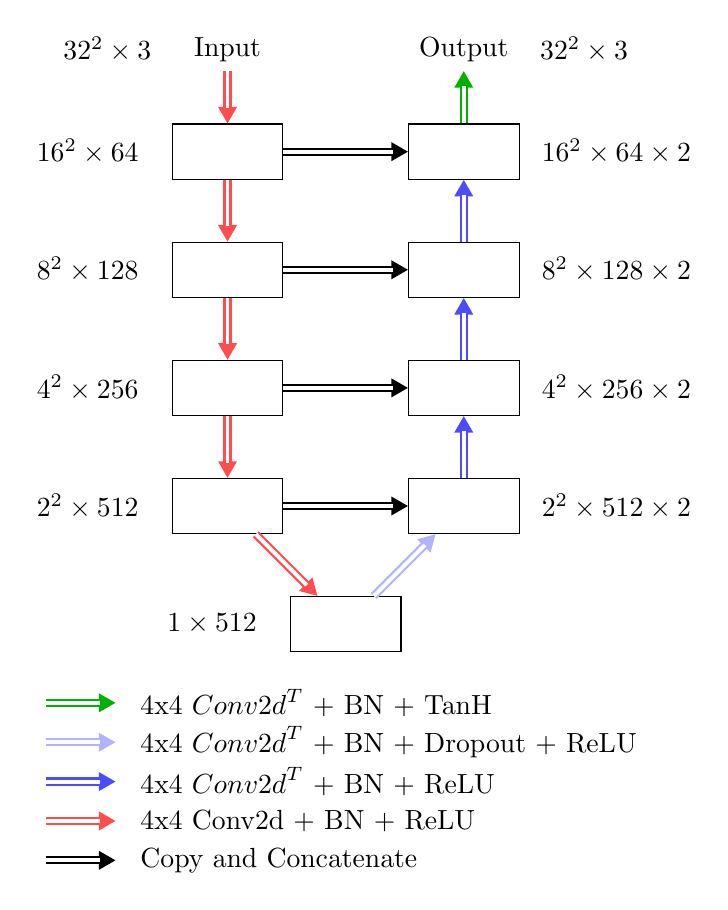
\begin{tikzpicture}

  \node (e0) at (-4,8.3)  {Input} ;
  \node[left = of e0, xshift=2em] {$32^2 \times 3$};
  \node (e1) at (-4,7)   [draw, minimum width=4em, minimum height=2em] {};
  \node[left = of e1, xshift=2em] {$16^2 \times 64$};
  \node (e2) at (-4,5.5) [draw, minimum width=4em, minimum height=2em] {};
  \node[left = of e2, xshift=2em] {$8^2 \times 128$};
  \node (e3) at (-4,4)   [draw, minimum width=4em, minimum height=2em] {};
  \node[left = of e3, xshift=2em] {$4^2 \times 256$};
  \node (e4) at (-4,2.5) [draw, minimum width=4em, minimum height=2em] {};
  \node[left = of e4, xshift=2em] {$2^2 \times 512$};

  \node (b)  at (-2.5,1) [draw, minimum width=4em, minimum height=2em] {};
  \node[left = of b, xshift=2em] {$1 \times 512$};

  \node (d0) at (-1,8.3) {Output};
  \node[right = of d0, xshift=-2.4em] {$32^2 \times 3$};
  \node (d1) at (-1,7)   [draw, minimum width=4em, minimum height=2em] {};
  \node[right = of d1, xshift=-2.4em] {$16^2 \times 64\times 2$};
  \node (d2) at (-1,5.5) [draw, minimum width=4em, minimum height=2em] {};
  \node[right = of d2, xshift=-2.4em] {$8^2 \times 128\times 2$};
  \node (d3) at (-1,4)   [draw, minimum width=4em, minimum height=2em] {};
  \node[right = of d3, xshift=-2.4em] {$4^2 \times 256\times 2$};
  \node (d4) at (-1,2.5) [draw, minimum width=4em, minimum height=2em] {};
  \node[right = of d4, xshift=-2.4em] {$2^2 \times 512\times 2$};

  \draw[vecArrow=red!70] (e0) -- (e1);
  \draw[vecArrow=red!70] (e1) -- (e2);
  \draw[vecArrow=red!70] (e2) -- (e3);
  \draw[vecArrow=red!70] (e3) -- (e4);

  \draw[vecArrow=red!70] (e4) -- (b);
  \draw[vecArrow=blue!30] (b)  -- (d4);

  \draw[vecArrow=blue!70] (d4) -- (d3);
  \draw[vecArrow=blue!70] (d3) -- (d2);
  \draw[vecArrow=blue!70] (d2) -- (d1);
  \draw[vecArrow=green!70!black] (d1) -- (d0);

  \draw[vecArrow] (e1) -- (d1);
  \draw[vecArrow] (e2) -- (d2);
  \draw[vecArrow] (e3) -- (d3);
  \draw[vecArrow] (e4) -- (d4);

  
  \node[] (n0) at (-5.3,-2) {};
  \node[right = of n0, xshift=-3em] {Copy and Concatenate};
  \draw[vecArrow] (-6.3,-2) -- (n0);

  \node[] (n1) at (-5.3,-1.5) {};
  \node[right = of n1, xshift=-3em] {4x4 Conv2d + BN + ReLU};
  \draw[vecArrow=red!70] (-6.3,-1.5)   -- (n1);

  \node[] (n2) at (-5.3,-1) {};
  \node[right = of n2, xshift=-3em] {4x4 $\text{Conv2d}^T$ + BN + ReLU} ;
  \draw[vecArrow=blue!70] (-6.3,-1) -- (n2);

  \node[] (n3) at (-5.3,-.5) {};
  \node[right = of n3, xshift=-3em] {4x4 $\text{Conv2d}^T$ + BN + Dropout + ReLU} ;
  \draw[vecArrow=blue!30] (-6.3,-.5)   -- (n3)  ;

  \node[] (n4) at (-5.3,0) {};
  \node[right = of n4, xshift=-3em]{4x4 $\text{Conv2d}^T$ + BN + TanH};
  \draw[vecArrow=green!70!black] (-6.3,0) -- (n4);
\end{tikzpicture}
\caption{Diagram of the U-net architecture}
\label{fig:unet}
  \vspace{4mm}
\end{figure}